\documentclass[journal,twoside,web]{ieeecolor}
\usepackage{generic}
\usepackage{cite}
\usepackage{amsmath,amssymb,amsfonts}
\usepackage{algorithmic}
\usepackage{graphicx}
\usepackage{algorithm,algorithmic}
\usepackage{hyperref}
\hypersetup{hidelinks=true}
\usepackage{textcomp}
% added packages
\usepackage{subcaption}
\graphicspath{{Fig/}}
\usepackage{booktabs}
\usepackage[flushleft]{threeparttable}
\usepackage{placeins}
%\usepackage{natbib}
\usepackage{subcaption}
\graphicspath{{Fig/}}
\usepackage{booktabs}
\usepackage[flushleft]{threeparttable}
\usepackage{placeins}

%cover letter
%https://docs.google.com/document/d/1LAgpGCCsmZacDEMiExaObtIIpZEOBkV-/edit?usp=sharing&ouid=113013698888183690561&rtpof=true&sd=true


\def\BibTeX{{\rm B\kern-.05em{\sc i\kern-.025em b}\kern-.08em
    T\kern-.1667em\lower.7ex\hbox{E}\kern-.125emX}}
\markboth{\hskip25pc IEEE TRANSACTIONS AND JOURNALS TEMPLATE}
{Author \MakeLowercase{\textit{et al.}}: Title}
\begin{document}
\title{Supplementary material for\\ DruGNNosis-MoA: Elucidating Drug Mechanisms as Etiological or Palliative With Graph Neural Networks Employing a Large Language Model}
\author{Brettler Liad, 
Berman Eden,
Jagodnik Kathleen M.,
and 
Bartal Alon
%\thanks{This paragraph of the first footnote will contain the date on 
%which you submitted your paper for review. It will also contain support information, including sponsor and financial support acknowledgment. 
%For example, ``This work was supported in part by the U.S. Department of Commerce under Grant 123456.'' }
\thanks{
All authors are with the The School of Business Administration, Bar-Ilan University, Ramat-Gan, 5290002, Israel (e-mail: alon.bartal@biu.ac.il).}
%\thanks{Second B. Author Jr. was with Rice University, Houston, TX 77005 USA. He is 
%now with the Department of Physics, Colorado State University, Fort Collins, 
%CO 80523 USA (e-mail: author@lamar.colostate.edu).}
%\thanks{Third C. Author is with 
%the Electrical Engineering Department, University of Colorado, Boulder, CO 
%80309 USA, on leave from the National Research Institute for Metals, 
%Tsukuba, Japan (e-mail: author@nrim.go.jp).}
}

\maketitle

%Full names of authors are preferred in 

%the author field, but are not required.

%Put a space between authors' initials.

%The abstract must be between 150--250 words. 

% three or four different keywords or phrase

%---------------------------------------------------------------------
\appendices
%---------------------------------------------------------------------
%\begin{appendices}

\setcounter{figure}{0}
\renewcommand\thefigure{S\arabic{figure}} % Redefine table numbering style

\section{Supplementary Tables}
\label{sec11}
%-------------------
\subsection{Supplementary Table S1}
Tab 1 of the Supplementary Table S1 contains the supplementary materials related to the drug mechanism annotations and can be accessed through the GitHub repository located at: \url{https://github.com/bartala/PalliativEtiological/tree/main/Supplementary}.

%-------------------
%\subsection{Supplementary Table S2}
%-------------------
Tab 2 of the Supplementary Table S1 contains the supplementary materials related to the example drug mechanism and can be accessed through the GitHub repository located at \url{https://github.com/bartala/PalliativEtiological/tree/main/Supplementary}.

%-------------------
\section{Supplementary Figures}
%-------------------
\begin{figure}[H]
    \centering
    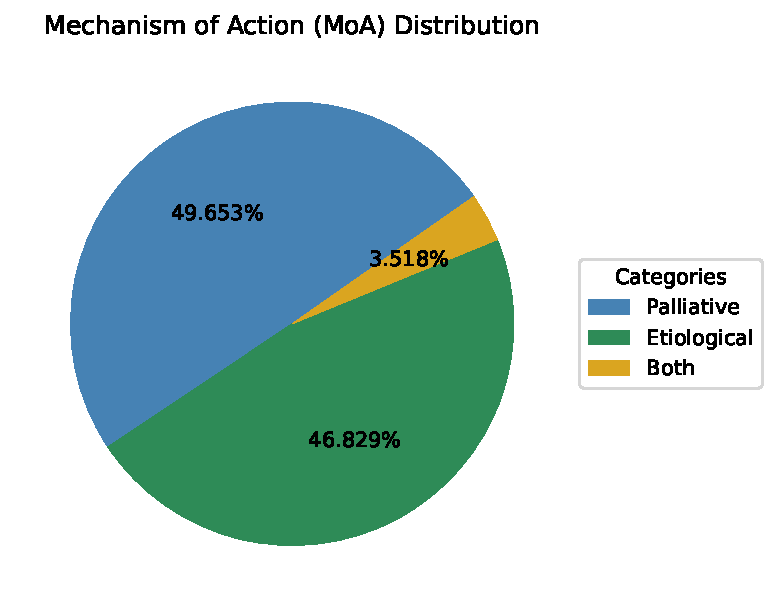
\includegraphics[width=\linewidth]{Figures/EvsP.pdf}
    \caption{Distribution of drug mechanisms of action. The number of etiological and palliative drugs is well balanced, with 47.423\% (957) being etiological, and 48.761\% (984) being palliative.
    Only a small percentage (3.816\%, 77) of drugs exhibit both mechanisms.}
    \label{fig:EvsP}
\end{figure}


%-------------------
%\section{Supplementary Fig. D: Distribution of drug mechanisms across Anatomical Therapeutic Chemical (ATC) classes}
%-------------------
\begin{figure}[H]
    \centering
    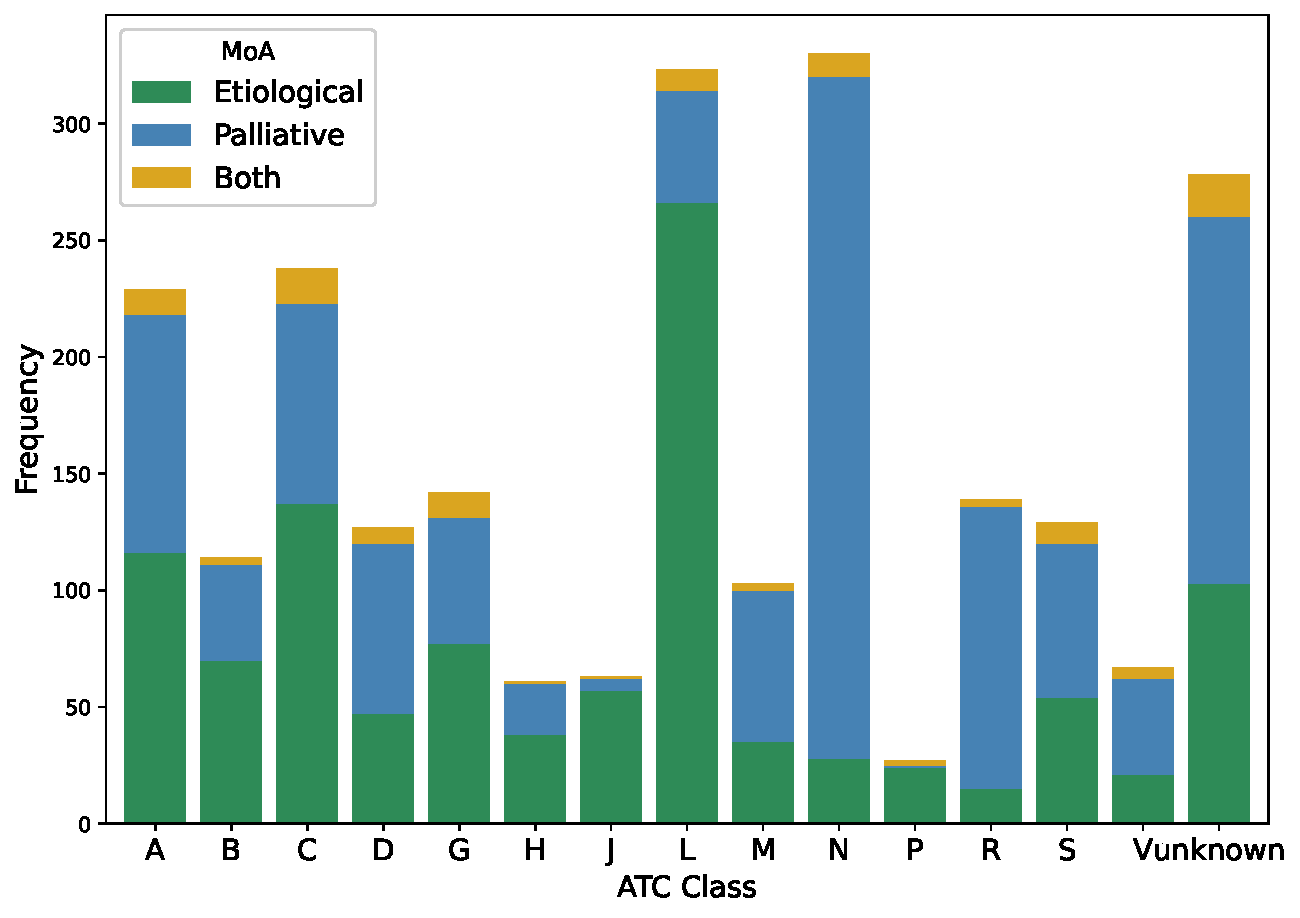
\includegraphics[width=\linewidth]{Figures/EPvsATC.pdf}
    \caption{ Distribution of drug mechanisms across Anatomical Therapeutic Chemical (ATC) classes.
    Each ATC class has a unique distribution of drug mechanisms.
    Some classes, e.g., `J', `L', and `P', are mainly associated with drugs having etiological mechanisms.
    In contrast, classes like 'N' and `R' are primarily associated with drugs having palliative mechanisms.
    The remaining classes generally exhibit a balance between drugs with etiological and palliative mechanisms.
    ATC Class Definitions:
   ``A": Alimentary tract and metabolism;
   ``B": Blood and blood forming organs;
   ``C": Cardiovascular system;
   ``D": Dermatologicals;
   ``G": Genito urinary system and sex hormones;
   ``H": Systemic hormonal preparations, excluding sex hormones and insulins;
   ``J": Antiinfectives for systemic use;
   ``L": Antineoplastic and immunomodulating agents;
   ``M": Musculo-skeletal system;
   ``N": Nervous system;
   ``P": Antiparasitic products, insecticides and repellents;
   ``R": Respiratory system;
   ``S": Sensory organs;
   ``V": Various;
   "Unknown": Drug entries that do not have an ATC class assigned to them in DrugBank.
    }
    \label{fig:EPvsATC}
\end{figure}


%-------------------
%\section{Supplementary Fig. E: Comprehensive overview of the F1-score performance of three models developed in this study to classify drugs as having etiological or palliative mechanism}
%-------------------

\begin{figure}[H]
\centering
\begin{subfigure}[H]{\linewidth}
   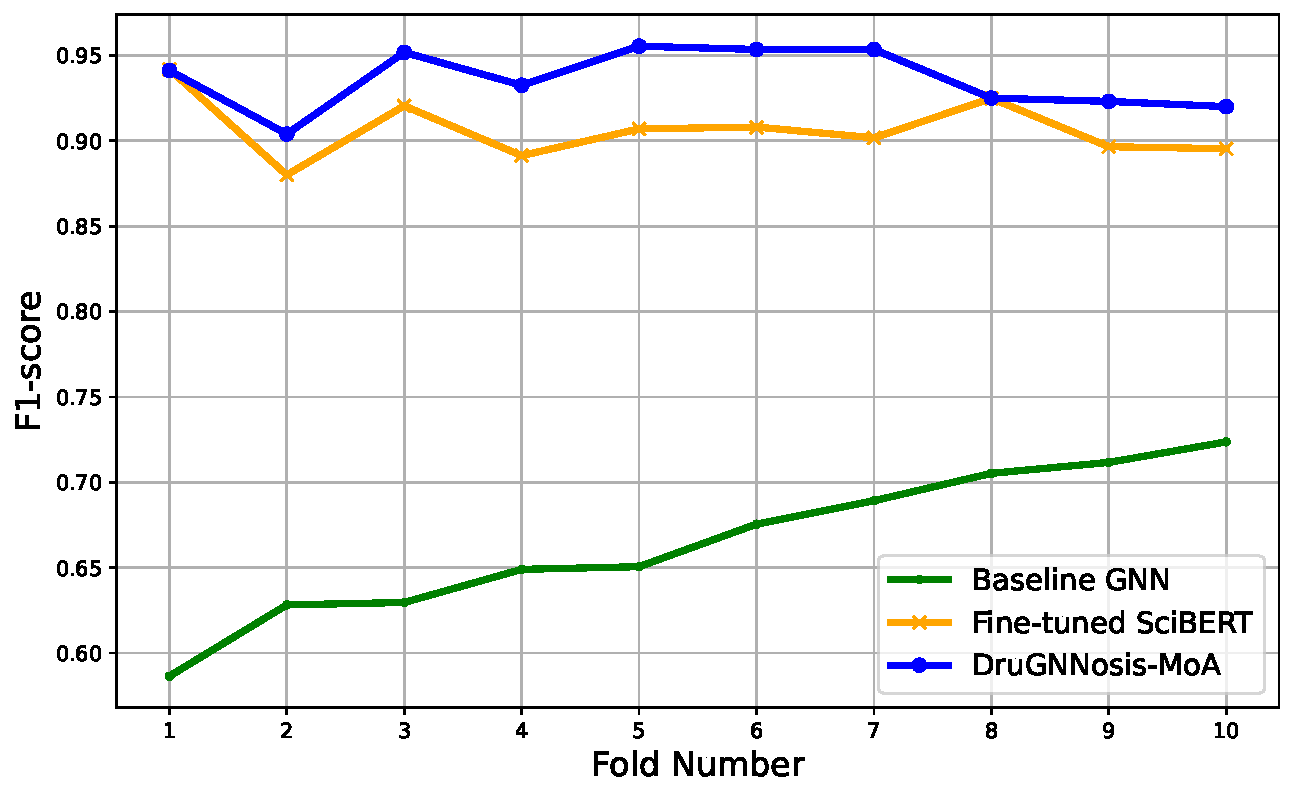
\includegraphics[width=\linewidth]{Figures/Comparison_F1_Scores_3_models.pdf}
   \caption{Comprehensive overview of the F1-score performance of three models developed in this study to classify drugs as having etiological or palliative mechanism.
   The results of the Baseline GNN model are characterized by an average F1-score of 0.664 and standard deviation of 0.043.
   Among the three models, the Baseline GNN model exhibits the lowest performance.
   The blue line represents our DruGNNosis-MoA model, the orange line represents the SciBERT model \citep{beltagy2019scibert}, and the green line represents the Baseline GNN model.}
   \label{fig:fscore1a}
\end{subfigure}
\begin{subfigure}[H]{\linewidth}
   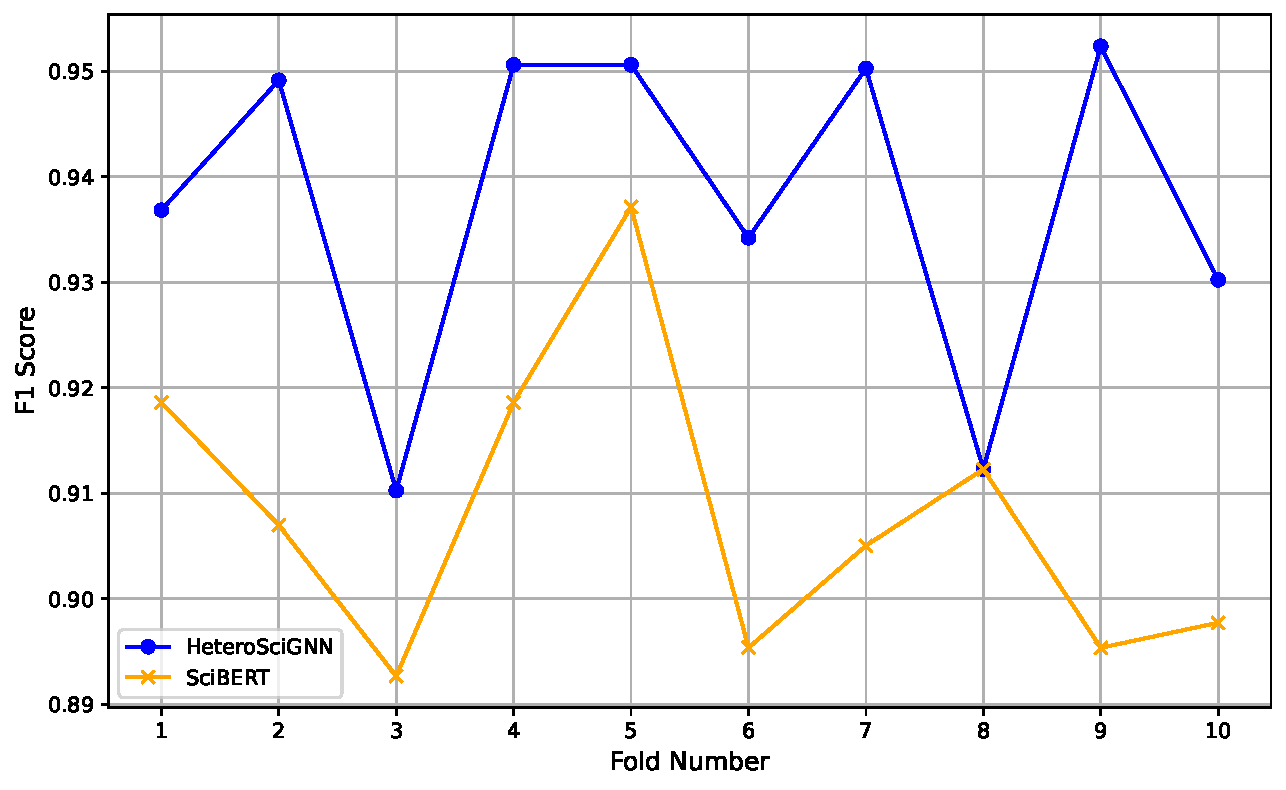
\includegraphics[width=\linewidth]{Figures/Comparison_F1_Scores_2_models.pdf}
   \caption{Comparison of F1-scores between the DruGNNosis-MoA and SciBERT models.
   Each point on the lines corresponds to the F1-score obtained for that particular fold of the cross-validation.
   There is a clear observation that the DruGNNosis-MoA model performed better on a fold-by-fold basis.}
   \label{fig:fscore1b}
\end{subfigure}
\caption{F1-score comparisons for different models.}
\label{fig:fscore1}
\end{figure}



%-------------------
%\section{Supplementary Fig. F: Receiver operating characteristic (ROC) curve of three models to classify drugs as having etiological or palliative mechanism}
%-------------------

\begin{figure}[H]
\centering
\begin{subfigure}[H]{\linewidth}
   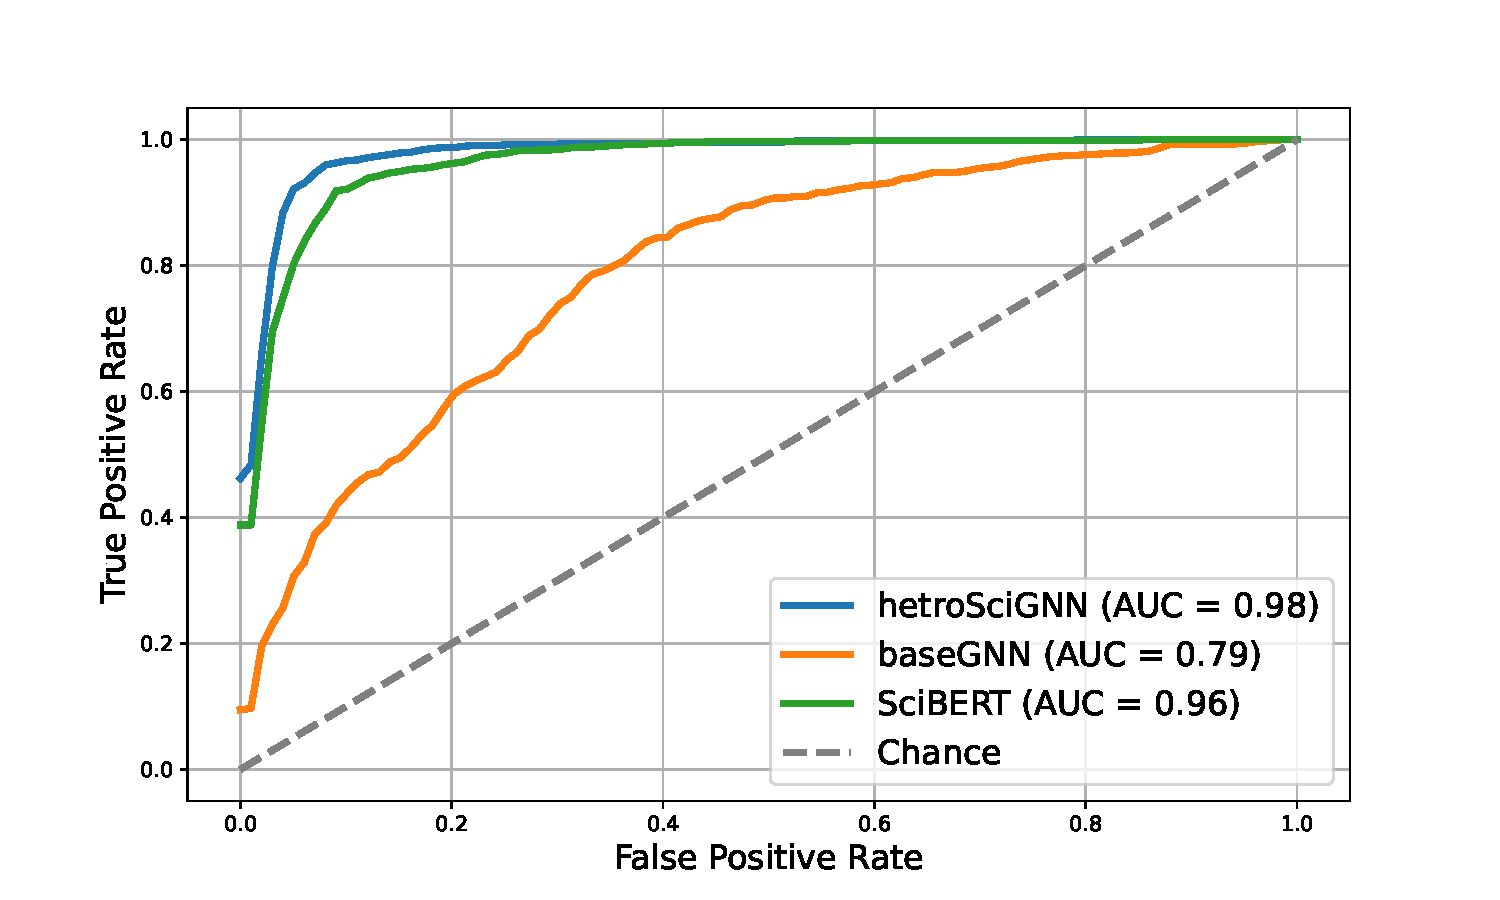
\includegraphics[width=\linewidth]{Figures/3_Models_Roc.pdf}
   \caption{
    Receiver operating characteristic (ROC) curve of three models to classify drugs as having etiological or palliative mechanism.
    The ROC curve compares the performance of three models over 10-fold cross-validation: Baseline GNN (blue), Fine-tuned SciBERT (orange), and DruGNNosis-MoA (green).
    Each line denotes the average ROC- Area Under Curve (AUC) for a model, indicating its True Positive Rate against the False Positive Rate.
    The dashed line represents the performance of a random (by chance) classifier, for reference.}
   \label{fig:roc_auc1a}
\end{subfigure}
\begin{subfigure}[H]{\linewidth}
   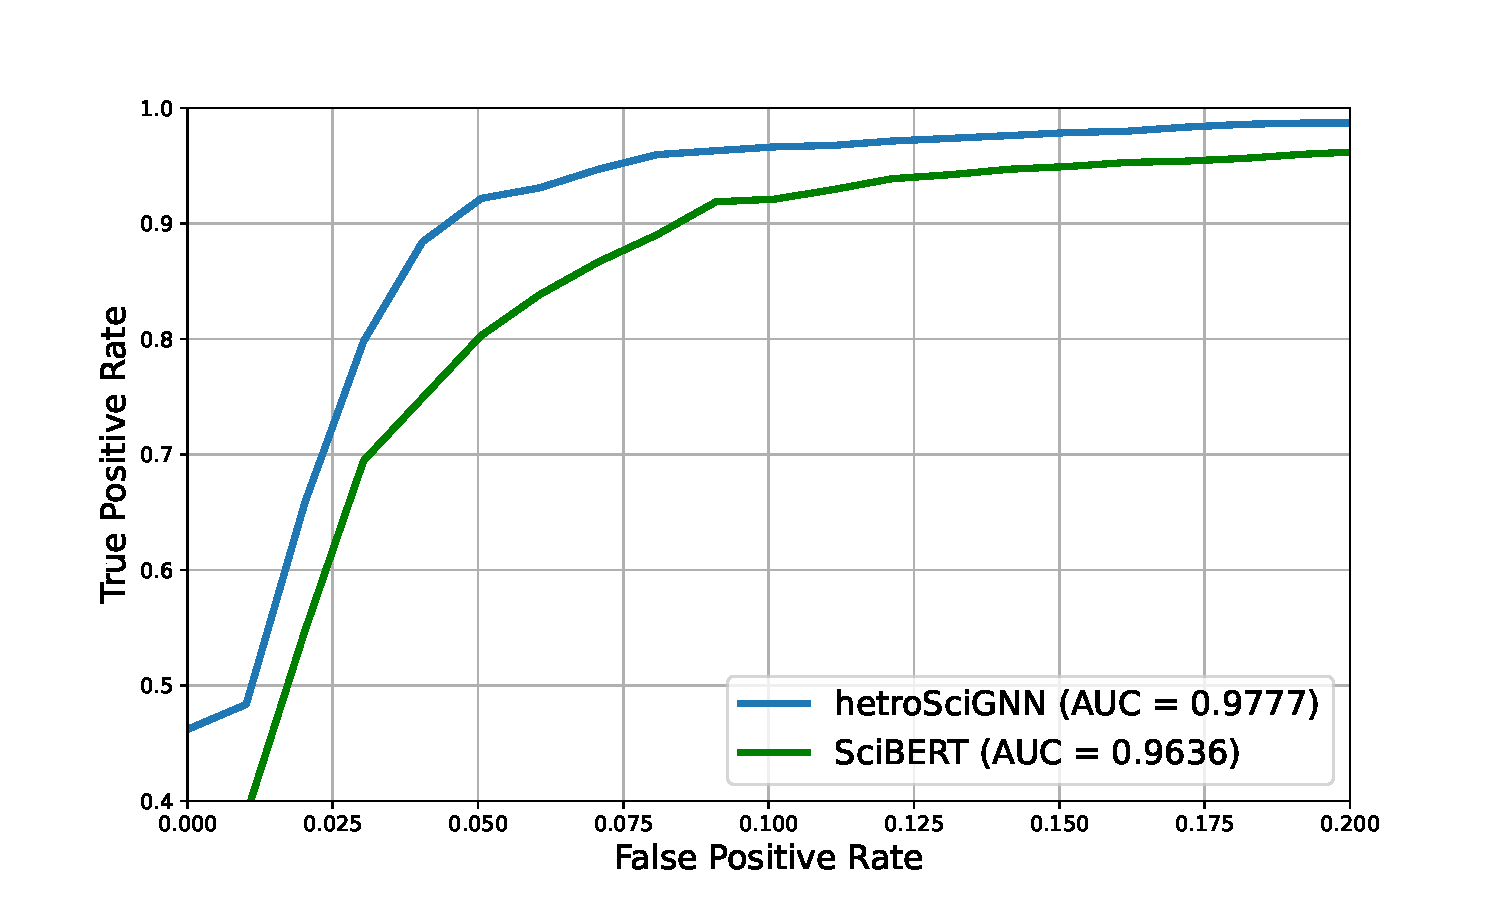
\includegraphics[width=\linewidth]{Figures/LLM_GNN_ROC_AUC.pdf}
   \caption{
    ROC curve highlighting the performance of the two top-performing models over 10-fold cross-validation: Fine-tuned SciBERT model (orange) and our DruGNNosis-MoA model (blue).
    Each line represents the average 10-fold CV ROC-AUC for a model, indicating its True Positive Rate (ranging from 0.4 to 1) against the False Positive Rate (ranging from 0 to 0.2).}
   \label{fig:roc_auc1b}
\end{subfigure}
\caption{Receiver Operating Characteristic (ROC) curves comparing the performance of three models to classify drugs as having etiological or palliative mechanism.}
\label{fig:roc_auc1}
\end{figure}



%-------------------
%\section{Supplementary Fig. G: All vs. All (Comprehensive) Method} 
%-------------------

\begin{figure}[H]
\centering
\begin{subfigure}[H]{\linewidth}
   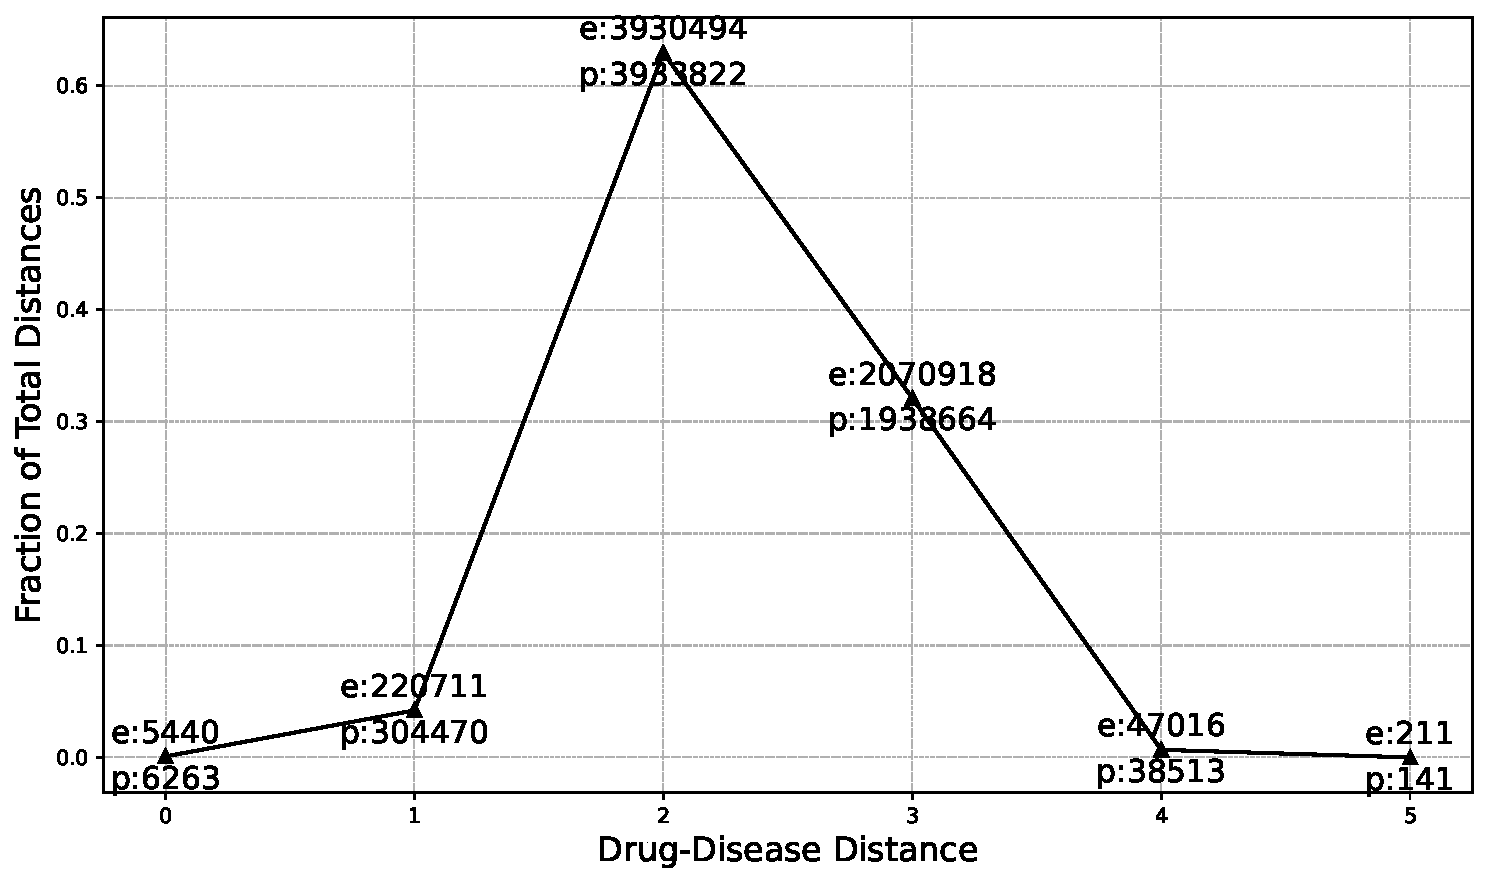
\includegraphics[width=\linewidth]{Figures/Yildrim_all_shortest_distance.pdf}
   \caption{\textbf{All vs. All (Comprehensive) Method:} Calculates and counts the shortest distance between each drug and disease pair, considering each occurrence of the drug in multiple paths.
   According to the technique of \cite{yildirim2007drug}, distances 0 and 1 hold statistical significance and are considered to indicate etiological drug mechanisms.}
   \label{fig:yildirim1}
\end{subfigure}
\begin{subfigure}[H]{\linewidth}
   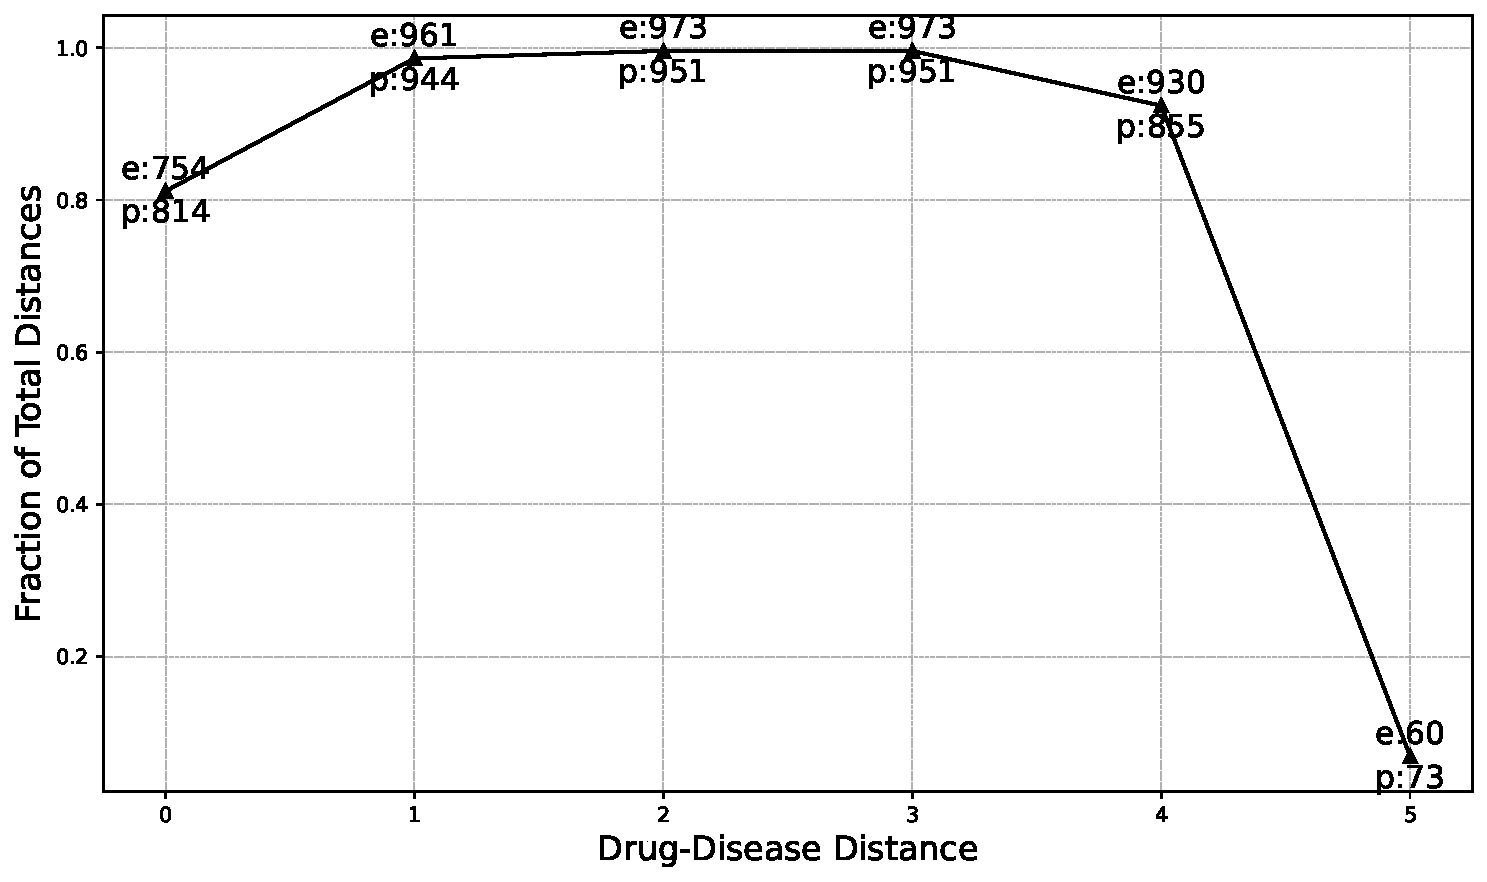
\includegraphics[width=\linewidth]{Figures/Yildrim_ALL_unique_drug_count_shortest_distance.pdf}
   \caption{\textbf{All vs. All (Unique) Method:} 
   Calculates the shortest distances between each drug and disease pair using a distinct counting mechanism. A drug is counted only once at each unique distance, regardless of how many times it appears at that distance. This ensures a balanced representation of drug applications relative to distance, preventing overemphasis on drugs appearing multiple times at the same distance.}
   \label{fig:yildirim2}
\end{subfigure}
\begin{subfigure}[H]{\linewidth}
   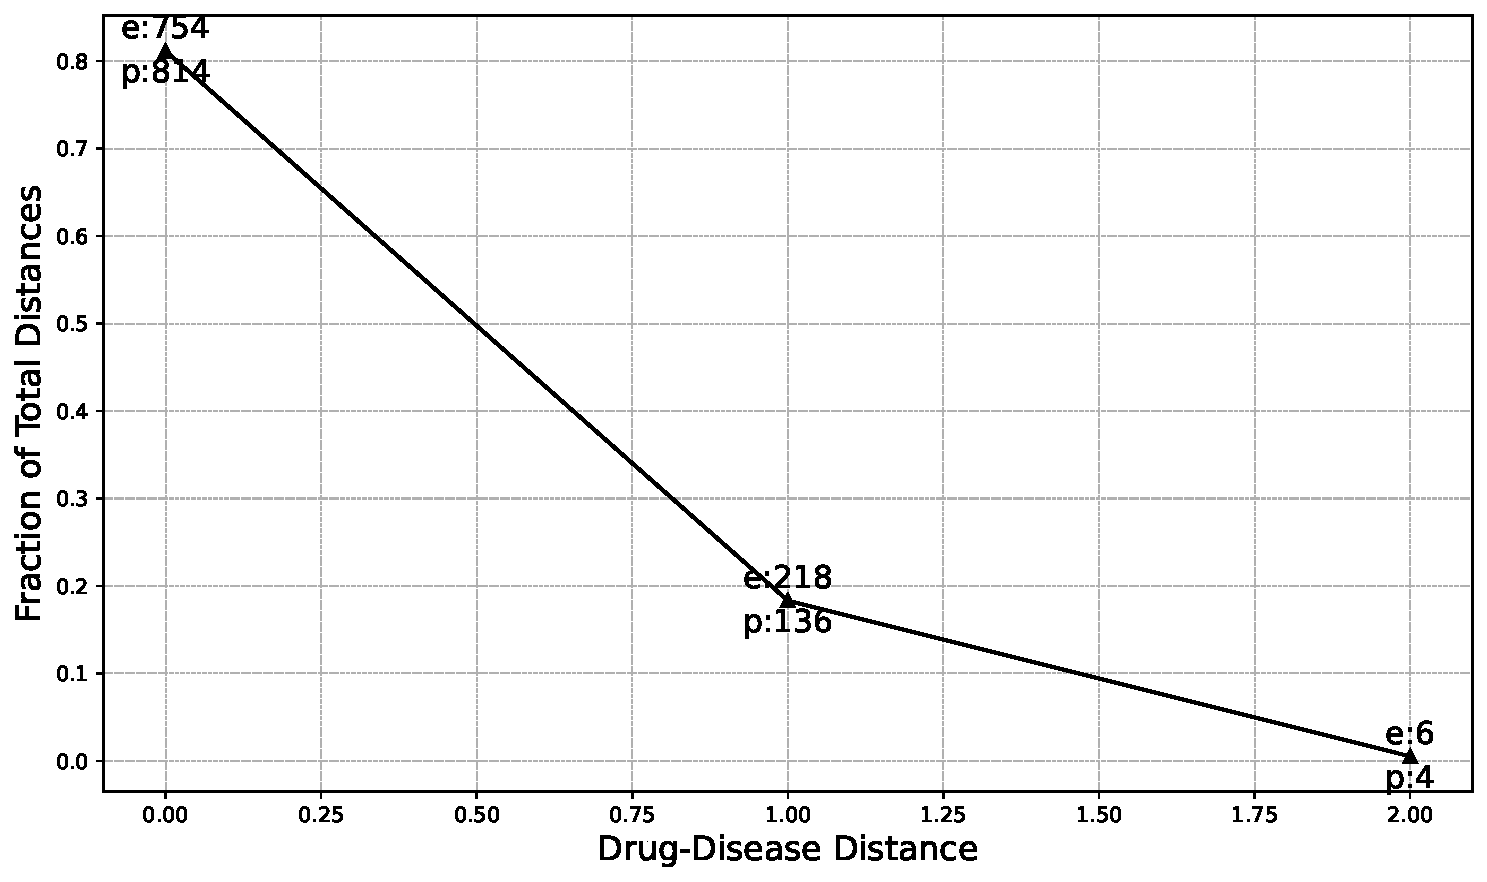
\includegraphics[width=\linewidth]{Figures/Yildrim_unique_minimum_shortest_distance.pdf}
   \caption{\textbf{Unique Minimum Shortest Distance Method:} 
   For each drug, we identified its shortest distance to a disease. 
   If a drug had the same shortest distance to multiple diseases, we retained only one unique distance per drug, removing duplicates.
   }
   \label{fig:yildirim3}
\end{subfigure}
\caption{Three methods for calculating drug-disease distances.
%We refer to the methodology of \cite{yildirim2007drug}.
Abbreviations: e = Etiological, p = Palliative. 
Numerical values represent the number of paths between drug and disease pairs at a specific distance. 
The fraction for each distance (path length) is calculated by dividing the number of occurrences of that specific path length by the total number of paths in the dataset.
This measures how common each distance is, relative to all possible paths.}
\label{fig:yildirim}
\end{figure}

%\end{appendices}

\end{document}
